%%%%%%%%%%%%%%%%%%%%%%%%%%%%%%%%%%%%%%%%%
% JPL Scientist IV Research Statement
% Derived from main.tex in this directory.
%%%%%%%%%%%%%%%%%%%%%%%%%%%%%%%%%%%%%%%%%

\documentclass[11pt,letterpaper,sans]{moderncv}

\moderncvstyle{casual}
\moderncvcolor{grey}

\usepackage[scale=0.83]{geometry}
\usepackage[hidelinks]{hyperref}
\usepackage{enumitem}
\setlist[itemize]{leftmargin=1.2em,itemsep=0.2em,topsep=0.2em}
\setlength{\hintscolumnwidth}{2.0cm}
\setlength{\footskip}{41pt}
\newcommand{\fieldlevelfigure}{%
\begin{center}
\vspace{-0.3em}
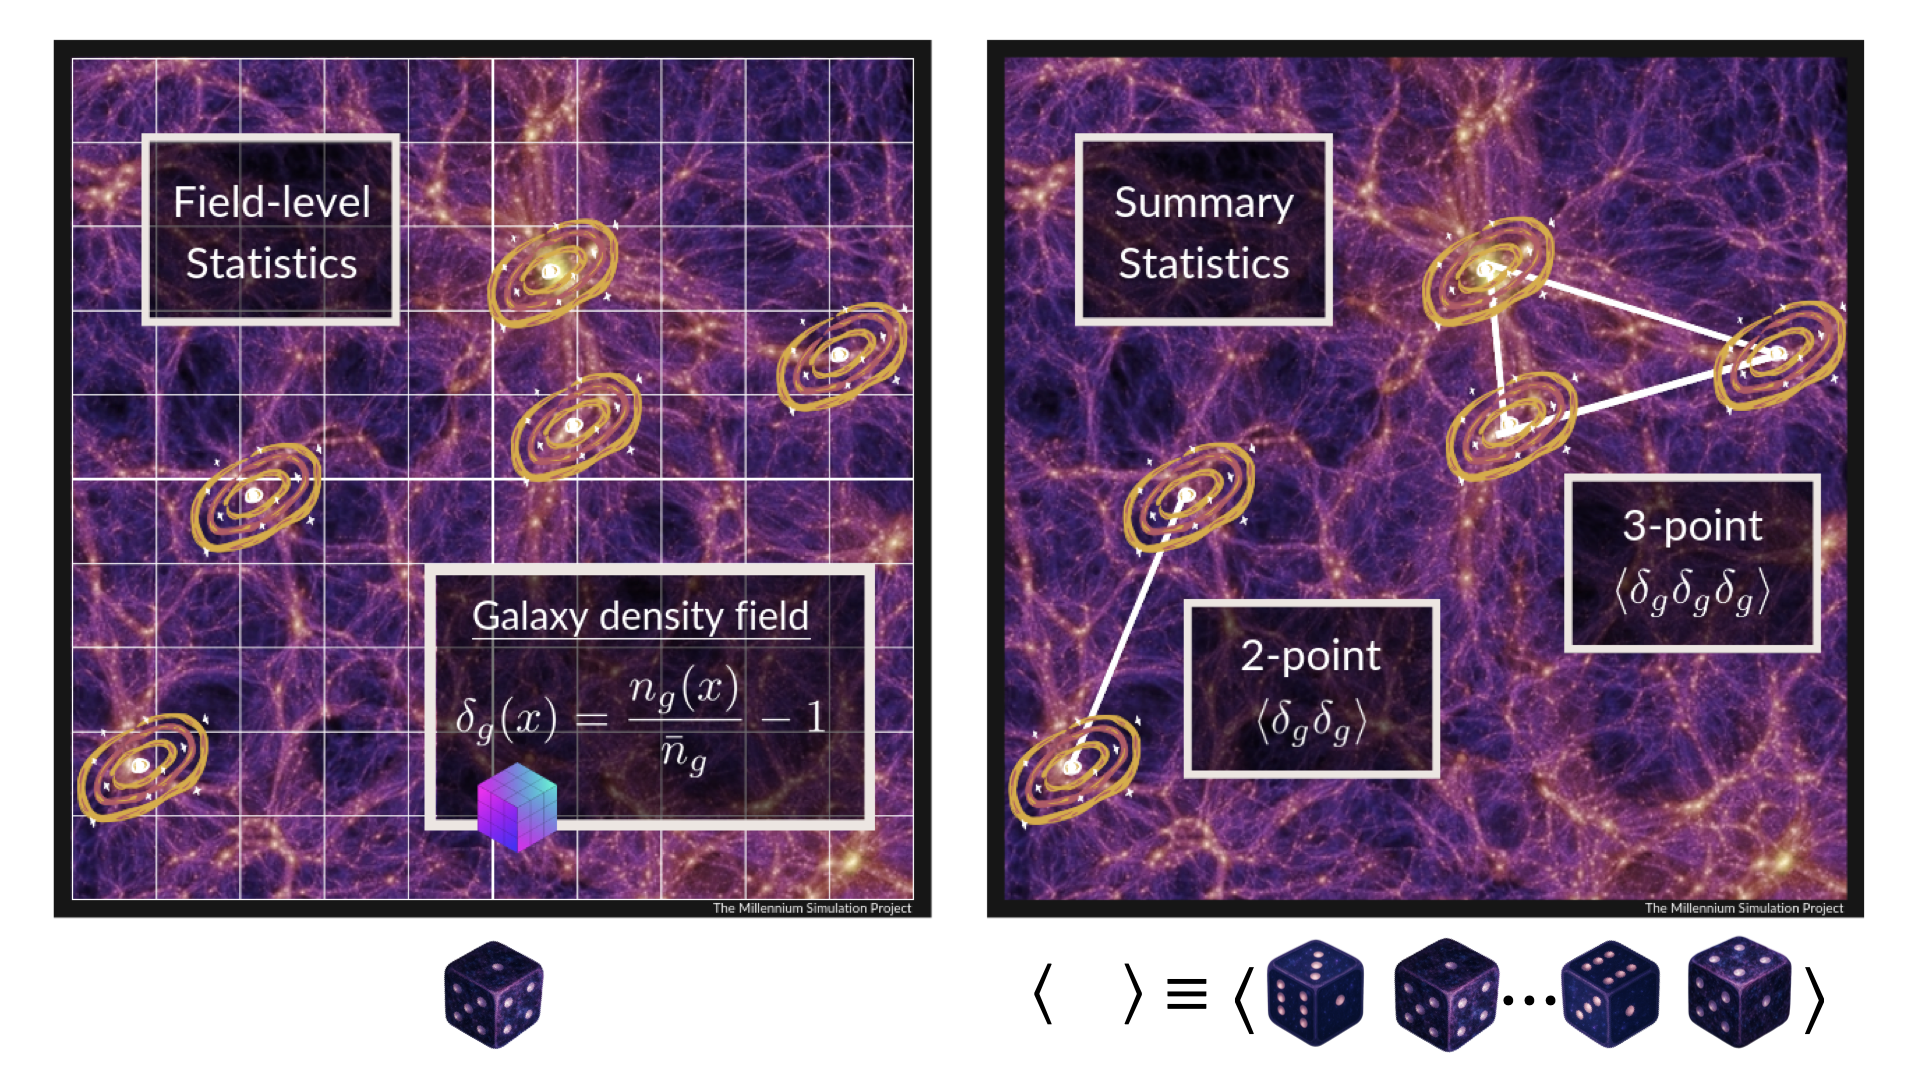
\includegraphics[width=0.68\textwidth]{figures/FLI_vs_2+3-point.png}\\[-0.2em]
{\footnotesize Field-level analyses preserve the observed galaxy field, while summary statistics compress it into low-order correlation functions.}
\vspace{-0.8em}
\end{center}}

\firstname{Nhat-Minh}
\familyname{Nguyen}
\title{Research Statement: Scientist IV, Roman and Euclid Cosmology}
\address{Kavli Institute for the Physics and Mathematics of the Universe}{University of Tokyo}
\email{nhat.minh.nguyen@ipmu.jp}
\homepage{https://minhmpa.github.io/}

\begin{document}
\makecvtitle
\vspace{-1.2em}

\section{Research vision}
My research is driven by a simple question: what is the optimal representation of galaxy-survey data for the physics we want to test? For Roman and Euclid, that question becomes urgent. Their weak-lensing and galaxy-clustering measurements will be precise enough that the limiting uncertainty will often be our modeling: how well we connect images, redshifts, selection functions, intrinsic alignments, galaxy bias, and nonlinear structure to statements about dark matter, dark energy, and gravity.

I work on field-level and forward-modeling methods for large-scale-structure cosmology. My specific niche is likelihood validation and information accounting: choosing the data representation that is optimal for a given physical question, then testing where that likelihood compresses information or becomes biased. At the Jet Propulsion Laboratory (JPL), I would use this background to help build a Roman--Euclid validation program that compares weak-lensing, clustering, and cross-survey information under controlled theoretical assumptions. The goal is not to replace standard mission analyses. The goal is to know when they are sufficient, when they are fragile, and when higher-order or field-level information changes a dark-sector conclusion.

\section{Preparation: growth, field-level inference, and survey realism}
My preparation connects three pieces that matter for this role: growth of structure as a dark-sector test, field-level inference as an accounting tool, and survey realism as the condition that makes either one useful.

The science driver is growth. My first-author Physical Review Letters (PRL) paper reported evidence for a late-time suppression in the growth of large-scale structure using a growth-index framework, combining information from the cosmic microwave background (CMB), weak lensing, galaxy clustering, and cosmic velocities. With collaborators, I later connected this phenomenology to modified-gravity parameterizations. That work shaped how I read survey data: a tension is interesting only after the modeling assumptions are visible.

The technical path is field-level inference. I develop Bayesian forward-modeling methods that infer cosmology from the observed realization of large-scale structure, rather than only from low-order summaries. In a first-author PRL with collaborators, I quantified how much information nonlinear galaxy clustering contains at the field level using LEFTfield, an effective-field-theory (EFT) differentiable forward model. This work was recognized by the 2024 Buchalter Cosmology Prize.

\fieldlevelfigure

For Roman and Euclid, I see field-level inference first as a validation tool. It can test information loss, stress-test scale cuts, expose model misspecification, and show when higher-order or field-level information changes the answer. That is the bridge from method development to mission analysis.

The practical bridge is survey realism. In the Prime Focus Spectrograph (PFS), I am responsible for the full-shape galaxy-clustering analysis pipeline. My single-author 2026 arXiv preprint, submitted to JCAP, ``Multi-tracers, multi-surveys: a joint Fisher analysis of DESI+PFS,'' grows from that pipeline and studies how survey overlap and multiple tracers calibrate full-shape nuisance parameters for PFS and the Dark Energy Spectroscopic Instrument (DESI). My work on field-level inference of galaxy intrinsic alignment from Sloan Digital Sky Survey Baryon Oscillation Spectroscopic Survey galaxy samples connects galaxy shapes, tidal fields, and weak-lensing systematics. My lensing-facing contribution is not shear-production ownership; it is the ability to stress-test the cosmology-facing connections among calibrated shape catalogs, photometric-redshift information, clustering data, and mission mocks.

\section{Proposed JPL research program}
At JPL, I would build around three connected directions.

\textbf{Joint weak-lensing and clustering inference.} Weak lensing measures projected matter; galaxy clustering measures biased tracers in three dimensions. The two probes are most powerful when their nuisance parameters are modeled together. I would develop diagnostics that treat matter clustering, tracer bias, intrinsic alignment, survey selection, and cross-probe covariance as coupled parts of one inference problem. In particular, I would test how intrinsic-alignment modeling, photometric-redshift leakage into lensing--clustering cross-correlations, source--lens coupling, and cross-covariance with clustering move the inferred growth signal. These diagnostics would sit downstream of existing shear, photo-z, and clustering products: not replacing production pipelines, but asking how their residual uncertainties enter dark-sector inference. The output should be practical: which Roman and Euclid observables give the cleanest tests of growth and gravity, and which assumptions still control the error budget.

\textbf{Roman--Euclid cross-calibration and simulation-based validation.} The overlap between Roman and Euclid is a calibration laboratory. I would make this concrete through mock challenges: inject blending, photometric-redshift, intrinsic-alignment, and selection perturbations into Roman--Euclid-like mocks; analyze them with matched summary-statistic, higher-order, and field-level or forward-modeled likelihoods; and measure which systematics self-calibrate from overlap data, which require external priors, and which propagate into dark-energy or modified-gravity constraints. Roman's depth and image quality can anchor the faint-galaxy and blending side of this test. Euclid supplies the area.

\textbf{Dark-sector interpretation from controlled modeling errors.} The payoff is not a smaller error bar by itself. It is a more trustworthy answer to whether geometry and growth agree. I would use Roman and Euclid weak-lensing and clustering measurements to build consistency tests for growth, gravitational slip, modified-gravity phenomenology, and dark-energy evolution. My field-level work would enter as a validation framework: compare summary-statistic, higher-order, and field-level analyses on the same mocks; quantify information loss; and define model-error budgets before interpreting any tension as new physics.

\section{Scientist IV leadership and execution plan}
As a Scientist IV, I would aim to define a concrete JPL work package: a Roman--Euclid overlap mock challenge for likelihood validation and cross-calibration. In the first one to two years, I would integrate with the relevant Roman and Euclid analysis teams, identify the overlap validation problem with the highest mission value, and deliver shared mocks and diagnostics that connect weak lensing, clustering, and systematics. In years two to four, I would lead the validation analysis toward scale-cut and covariance recommendations, a documented likelihood-comparison product, and a dark-sector interpretation paper. By years four to five, I would aim to deliver community-facing validation products that support Roman early science and future survey-cosmology validation work.

My preparation for this role is technical and institutional. I have begun leading independent research through KAKENHI and astronomy research-support grants. I chaired the organizing committee for Beyond-2-Point Statistics Meet Survey Systematics and convened the large-scale-structure session at COSMO'24. I have also advised and co-mentored students and early-career researchers whose projects led to papers or accepted workshop publications. One example is Baptiste Barthe-Gold's density-field reconstruction project, which became an accepted NeurIPS 2025 ML4PS workshop publication.

That is also how I tend to work. I do not wait until I already know every piece of a problem; I build the first tractable version, use it to learn the missing pieces, and then make the result clear enough for other people to test or extend. At JPL, that habit would matter in a practical way: define the question sharply, make the validation reproducible, keep the interpretation conservative, and help younger scientists turn technical modules into durable collaboration products.

\section{Collaboration, mentoring, and inclusive team science}
The Roman and Euclid science return will depend on collaboration across mission teams, probe experts, simulation builders, theorists, and statisticians. I work best when those pieces have to meet. My role would be to connect nonlinear structure theory, likelihood validation, systematics propagation, and dark-sector phenomenology. I would make the work legible to the broader collaboration with clear documentation, shared benchmarks, and a sharp separation between robust conclusions and attractive but fragile ones.

I care about mentoring because difficult analyses survive only if people other than the original author can understand, test, and extend them. My experience co-mentoring, organizing journal clubs and seminars, and building international scientific programs has taught me that inclusive research culture is not separate from technical quality. The mentoring model I would bring is modular: help new collaborators start with a reproducible first contribution, let them own a validation module with explicit inputs and outputs, and then connect mature modules to papers or collaboration products. That model keeps expectations explicit, credit shared, and junior collaborators aware of how their technical contribution fits the mission-scale goal.

Roman and Euclid are where field-level and forward-modeling methods can become useful at mission scale. At JPL, I would use my background in growth, nonlinear modeling, field-level inference, and survey validation to help turn weak-lensing and clustering data into robust tests of dark matter, dark energy, and gravity.

\end{document}
